% Options for packages loaded elsewhere
\PassOptionsToPackage{unicode}{hyperref}
\PassOptionsToPackage{hyphens}{url}
\PassOptionsToPackage{dvipsnames,svgnames,x11names}{xcolor}
%
\documentclass[
  11pt,
  letterpaper,
  DIV=11,
  numbers=noendperiod]{scrartcl}

\usepackage{amsmath,amssymb}
\usepackage{iftex}
\ifPDFTeX
  \usepackage[T1]{fontenc}
  \usepackage[utf8]{inputenc}
  \usepackage{textcomp} % provide euro and other symbols
\else % if luatex or xetex
  \usepackage{unicode-math}
  \defaultfontfeatures{Scale=MatchLowercase}
  \defaultfontfeatures[\rmfamily]{Ligatures=TeX,Scale=1}
\fi
\usepackage{lmodern}
\ifPDFTeX\else  
    % xetex/luatex font selection
\fi
% Use upquote if available, for straight quotes in verbatim environments
\IfFileExists{upquote.sty}{\usepackage{upquote}}{}
\IfFileExists{microtype.sty}{% use microtype if available
  \usepackage[]{microtype}
  \UseMicrotypeSet[protrusion]{basicmath} % disable protrusion for tt fonts
}{}
\makeatletter
\@ifundefined{KOMAClassName}{% if non-KOMA class
  \IfFileExists{parskip.sty}{%
    \usepackage{parskip}
  }{% else
    \setlength{\parindent}{0pt}
    \setlength{\parskip}{6pt plus 2pt minus 1pt}}
}{% if KOMA class
  \KOMAoptions{parskip=half}}
\makeatother
\usepackage{xcolor}
\setlength{\emergencystretch}{3em} % prevent overfull lines
\setcounter{secnumdepth}{5}
% Make \paragraph and \subparagraph free-standing
\makeatletter
\ifx\paragraph\undefined\else
  \let\oldparagraph\paragraph
  \renewcommand{\paragraph}{
    \@ifstar
      \xxxParagraphStar
      \xxxParagraphNoStar
  }
  \newcommand{\xxxParagraphStar}[1]{\oldparagraph*{#1}\mbox{}}
  \newcommand{\xxxParagraphNoStar}[1]{\oldparagraph{#1}\mbox{}}
\fi
\ifx\subparagraph\undefined\else
  \let\oldsubparagraph\subparagraph
  \renewcommand{\subparagraph}{
    \@ifstar
      \xxxSubParagraphStar
      \xxxSubParagraphNoStar
  }
  \newcommand{\xxxSubParagraphStar}[1]{\oldsubparagraph*{#1}\mbox{}}
  \newcommand{\xxxSubParagraphNoStar}[1]{\oldsubparagraph{#1}\mbox{}}
\fi
\makeatother

\usepackage{color}
\usepackage{fancyvrb}
\newcommand{\VerbBar}{|}
\newcommand{\VERB}{\Verb[commandchars=\\\{\}]}
\DefineVerbatimEnvironment{Highlighting}{Verbatim}{commandchars=\\\{\}}
% Add ',fontsize=\small' for more characters per line
\usepackage{framed}
\definecolor{shadecolor}{RGB}{241,243,245}
\newenvironment{Shaded}{\begin{snugshade}}{\end{snugshade}}
\newcommand{\AlertTok}[1]{\textcolor[rgb]{0.68,0.00,0.00}{#1}}
\newcommand{\AnnotationTok}[1]{\textcolor[rgb]{0.37,0.37,0.37}{#1}}
\newcommand{\AttributeTok}[1]{\textcolor[rgb]{0.40,0.45,0.13}{#1}}
\newcommand{\BaseNTok}[1]{\textcolor[rgb]{0.68,0.00,0.00}{#1}}
\newcommand{\BuiltInTok}[1]{\textcolor[rgb]{0.00,0.23,0.31}{#1}}
\newcommand{\CharTok}[1]{\textcolor[rgb]{0.13,0.47,0.30}{#1}}
\newcommand{\CommentTok}[1]{\textcolor[rgb]{0.37,0.37,0.37}{#1}}
\newcommand{\CommentVarTok}[1]{\textcolor[rgb]{0.37,0.37,0.37}{\textit{#1}}}
\newcommand{\ConstantTok}[1]{\textcolor[rgb]{0.56,0.35,0.01}{#1}}
\newcommand{\ControlFlowTok}[1]{\textcolor[rgb]{0.00,0.23,0.31}{\textbf{#1}}}
\newcommand{\DataTypeTok}[1]{\textcolor[rgb]{0.68,0.00,0.00}{#1}}
\newcommand{\DecValTok}[1]{\textcolor[rgb]{0.68,0.00,0.00}{#1}}
\newcommand{\DocumentationTok}[1]{\textcolor[rgb]{0.37,0.37,0.37}{\textit{#1}}}
\newcommand{\ErrorTok}[1]{\textcolor[rgb]{0.68,0.00,0.00}{#1}}
\newcommand{\ExtensionTok}[1]{\textcolor[rgb]{0.00,0.23,0.31}{#1}}
\newcommand{\FloatTok}[1]{\textcolor[rgb]{0.68,0.00,0.00}{#1}}
\newcommand{\FunctionTok}[1]{\textcolor[rgb]{0.28,0.35,0.67}{#1}}
\newcommand{\ImportTok}[1]{\textcolor[rgb]{0.00,0.46,0.62}{#1}}
\newcommand{\InformationTok}[1]{\textcolor[rgb]{0.37,0.37,0.37}{#1}}
\newcommand{\KeywordTok}[1]{\textcolor[rgb]{0.00,0.23,0.31}{\textbf{#1}}}
\newcommand{\NormalTok}[1]{\textcolor[rgb]{0.00,0.23,0.31}{#1}}
\newcommand{\OperatorTok}[1]{\textcolor[rgb]{0.37,0.37,0.37}{#1}}
\newcommand{\OtherTok}[1]{\textcolor[rgb]{0.00,0.23,0.31}{#1}}
\newcommand{\PreprocessorTok}[1]{\textcolor[rgb]{0.68,0.00,0.00}{#1}}
\newcommand{\RegionMarkerTok}[1]{\textcolor[rgb]{0.00,0.23,0.31}{#1}}
\newcommand{\SpecialCharTok}[1]{\textcolor[rgb]{0.37,0.37,0.37}{#1}}
\newcommand{\SpecialStringTok}[1]{\textcolor[rgb]{0.13,0.47,0.30}{#1}}
\newcommand{\StringTok}[1]{\textcolor[rgb]{0.13,0.47,0.30}{#1}}
\newcommand{\VariableTok}[1]{\textcolor[rgb]{0.07,0.07,0.07}{#1}}
\newcommand{\VerbatimStringTok}[1]{\textcolor[rgb]{0.13,0.47,0.30}{#1}}
\newcommand{\WarningTok}[1]{\textcolor[rgb]{0.37,0.37,0.37}{\textit{#1}}}

\providecommand{\tightlist}{%
  \setlength{\itemsep}{0pt}\setlength{\parskip}{0pt}}\usepackage{longtable,booktabs,array}
\usepackage{calc} % for calculating minipage widths
% Correct order of tables after \paragraph or \subparagraph
\usepackage{etoolbox}
\makeatletter
\patchcmd\longtable{\par}{\if@noskipsec\mbox{}\fi\par}{}{}
\makeatother
% Allow footnotes in longtable head/foot
\IfFileExists{footnotehyper.sty}{\usepackage{footnotehyper}}{\usepackage{footnote}}
\makesavenoteenv{longtable}
\usepackage{graphicx}
\makeatletter
\newsavebox\pandoc@box
\newcommand*\pandocbounded[1]{% scales image to fit in text height/width
  \sbox\pandoc@box{#1}%
  \Gscale@div\@tempa{\textheight}{\dimexpr\ht\pandoc@box+\dp\pandoc@box\relax}%
  \Gscale@div\@tempb{\linewidth}{\wd\pandoc@box}%
  \ifdim\@tempb\p@<\@tempa\p@\let\@tempa\@tempb\fi% select the smaller of both
  \ifdim\@tempa\p@<\p@\scalebox{\@tempa}{\usebox\pandoc@box}%
  \else\usebox{\pandoc@box}%
  \fi%
}
% Set default figure placement to htbp
\def\fps@figure{htbp}
\makeatother

\KOMAoption{captions}{tableheading}
\makeatletter
\@ifpackageloaded{caption}{}{\usepackage{caption}}
\AtBeginDocument{%
\ifdefined\contentsname
  \renewcommand*\contentsname{Table of contents}
\else
  \newcommand\contentsname{Table of contents}
\fi
\ifdefined\listfigurename
  \renewcommand*\listfigurename{List of Figures}
\else
  \newcommand\listfigurename{List of Figures}
\fi
\ifdefined\listtablename
  \renewcommand*\listtablename{List of Tables}
\else
  \newcommand\listtablename{List of Tables}
\fi
\ifdefined\figurename
  \renewcommand*\figurename{Figure}
\else
  \newcommand\figurename{Figure}
\fi
\ifdefined\tablename
  \renewcommand*\tablename{Table}
\else
  \newcommand\tablename{Table}
\fi
}
\@ifpackageloaded{float}{}{\usepackage{float}}
\floatstyle{ruled}
\@ifundefined{c@chapter}{\newfloat{codelisting}{h}{lop}}{\newfloat{codelisting}{h}{lop}[chapter]}
\floatname{codelisting}{Listing}
\newcommand*\listoflistings{\listof{codelisting}{List of Listings}}
\makeatother
\makeatletter
\makeatother
\makeatletter
\@ifpackageloaded{caption}{}{\usepackage{caption}}
\@ifpackageloaded{subcaption}{}{\usepackage{subcaption}}
\makeatother
\makeatletter
\@ifpackageloaded{tcolorbox}{}{\usepackage[skins,breakable]{tcolorbox}}
\makeatother
\makeatletter
\@ifundefined{shadecolor}{\definecolor{shadecolor}{rgb}{.97, .97, .97}}{}
\makeatother
\makeatletter
\makeatother
\makeatletter
\ifdefined\Shaded\renewenvironment{Shaded}{\begin{tcolorbox}[breakable, frame hidden, enhanced, sharp corners, boxrule=0pt, interior hidden]}{\end{tcolorbox}}\fi
\makeatother

\usepackage{bookmark}

\IfFileExists{xurl.sty}{\usepackage{xurl}}{} % add URL line breaks if available
\urlstyle{same} % disable monospaced font for URLs
\hypersetup{
  pdftitle={Assignment 3 by Ctrl+Alt+Analyze},
  colorlinks=true,
  linkcolor={blue},
  filecolor={Maroon},
  citecolor={Blue},
  urlcolor={Blue},
  pdfcreator={LaTeX via pandoc}}


\title{Assignment 3 by Ctrl+Alt+Analyze}
\author{}
\date{}

\begin{document}
\maketitle

\renewcommand*\contentsname{Table of contents}
{
\hypersetup{linkcolor=}
\setcounter{tocdepth}{2}
\tableofcontents
}

\newpage

\begin{Shaded}
\begin{Highlighting}[]
\FunctionTok{library}\NormalTok{(}\StringTok{"here"}\NormalTok{)}
\FunctionTok{library}\NormalTok{(}\StringTok{"tidyverse"}\NormalTok{)}
\FunctionTok{library}\NormalTok{(}\StringTok{"ggplot2"}\NormalTok{)}
\FunctionTok{library}\NormalTok{(}\StringTok{"ggcorrplot"}\NormalTok{)}
\FunctionTok{library}\NormalTok{(}\StringTok{\textquotesingle{}readr\textquotesingle{}}\NormalTok{)}
\FunctionTok{library}\NormalTok{(}\StringTok{\textquotesingle{}corrplot\textquotesingle{}}\NormalTok{)}
\FunctionTok{library}\NormalTok{(}\StringTok{\textquotesingle{}tinytex\textquotesingle{}}\NormalTok{)}
\end{Highlighting}
\end{Shaded}

\begin{Shaded}
\begin{Highlighting}[]
\NormalTok{data }\OtherTok{\textless{}{-}} \FunctionTok{read\_csv}\NormalTok{(}\FunctionTok{here}\NormalTok{(}\StringTok{"data/student\_habits\_performance.csv"}\NormalTok{)) }

\CommentTok{\# renaming of things }
\NormalTok{good\_habits }\OtherTok{\textless{}{-}}\NormalTok{ data }\SpecialCharTok{|\textgreater{}}
  \FunctionTok{select}\NormalTok{(study\_hours\_per\_day, attendance\_percentage, sleep\_hours, exam\_score)}

\NormalTok{good\_cor\_matrix }\OtherTok{\textless{}{-}}\NormalTok{ good\_habits }\SpecialCharTok{|\textgreater{}}
  \FunctionTok{cor}\NormalTok{(}\AttributeTok{use =} \StringTok{"complete.obs"}\NormalTok{)}
\end{Highlighting}
\end{Shaded}

\section{Investigating the relationship between student's academic
performance and lifestyle
habits}\label{investigating-the-relationship-between-students-academic-performance-and-lifestyle-habits}

By Team : \textbf{Ctrl+Alt+Analyze}

Authors:

\begin{enumerate}
\def\labelenumi{\arabic{enumi}.}
\item
  Malaika
\item
  Zuxilu
\item
  Kunal
\end{enumerate}

\section{Executive summary}\label{executive-summary}

\begin{itemize}
\tightlist
\item
  This report investigates the relationship between student lifestyle
  habits and academic performance using correlation analysis. We
  classify study hours, class attendance, and sleep duration as ``good''
  habits, while the time spent on social media, and Netflix usage are
  treated as ``bad'' habits.
\item
  Our findings indicate that study hours have the strongest positive
  correlation with exam scores, while time spent on social media and
  Netflix show weak negative correlations. Results from our study can be
  used to guide and inform students about the relationship between their
  lifestyle choices and academic success.
\end{itemize}

\section{Introduction}\label{introduction}

Academic performance is influenced by a range of behavioral and
lifestyle factors. Habits such as consistent study routines, classroom
attendance, and adequate sleep are commonly associated with better exam
outcomes. In contrast, excessive time spent on social media and
streaming platforms may reduce focus and study time. This study aims to
quantify the relationship between these habits and academic performance
using correlation analysis. The dataset includes student-reported habits
and their corresponding exam scores. We define ``good habits'' as study
hours, class attendance, and sleep hours, and ``bad habits'' as social
media and Netflix usage. Using correlation matrices and visualizations,
we examine how each habit is associated with exam performance. Our goal
is to identify which habits have the strongest relationship with scores
and whether they are positive or negative. The findings may provide
insight into which behaviors support or hinder academic success. This
report is structured to include our methodology, results, discussion,
and recommendations.

\newpage

\section{Methodology}\label{methodology}

\begin{Shaded}
\begin{Highlighting}[]
\FunctionTok{library}\NormalTok{(knitr)}
\FunctionTok{kable}\NormalTok{(good\_cor\_matrix, }\AttributeTok{digits =} \DecValTok{2}\NormalTok{)}
\end{Highlighting}
\end{Shaded}

\begin{longtable}[]{@{}
  >{\raggedright\arraybackslash}p{(\linewidth - 8\tabcolsep) * \real{0.2529}}
  >{\raggedleft\arraybackslash}p{(\linewidth - 8\tabcolsep) * \real{0.2299}}
  >{\raggedleft\arraybackslash}p{(\linewidth - 8\tabcolsep) * \real{0.2529}}
  >{\raggedleft\arraybackslash}p{(\linewidth - 8\tabcolsep) * \real{0.1379}}
  >{\raggedleft\arraybackslash}p{(\linewidth - 8\tabcolsep) * \real{0.1264}}@{}}
\caption{Table 1: Correlation matrix of good habits and exam
score}\tabularnewline
\toprule\noalign{}
\begin{minipage}[b]{\linewidth}\raggedright
\end{minipage} & \begin{minipage}[b]{\linewidth}\raggedleft
study\_hours\_per\_day
\end{minipage} & \begin{minipage}[b]{\linewidth}\raggedleft
attendance\_percentage
\end{minipage} & \begin{minipage}[b]{\linewidth}\raggedleft
sleep\_hours
\end{minipage} & \begin{minipage}[b]{\linewidth}\raggedleft
exam\_score
\end{minipage} \\
\midrule\noalign{}
\endfirsthead
\toprule\noalign{}
\begin{minipage}[b]{\linewidth}\raggedright
\end{minipage} & \begin{minipage}[b]{\linewidth}\raggedleft
study\_hours\_per\_day
\end{minipage} & \begin{minipage}[b]{\linewidth}\raggedleft
attendance\_percentage
\end{minipage} & \begin{minipage}[b]{\linewidth}\raggedleft
sleep\_hours
\end{minipage} & \begin{minipage}[b]{\linewidth}\raggedleft
exam\_score
\end{minipage} \\
\midrule\noalign{}
\endhead
\bottomrule\noalign{}
\endlastfoot
study\_hours\_per\_day & 1.00 & 0.03 & -0.03 & 0.83 \\
attendance\_percentage & 0.03 & 1.00 & 0.01 & 0.09 \\
sleep\_hours & -0.03 & 0.01 & 1.00 & 0.12 \\
exam\_score & 0.83 & 0.09 & 0.12 & 1.00 \\
\end{longtable}

This study used correlation analysis to explore the relationship between
student habits and academic performance. The dataset included 100
student records with variables such as study hours, class attendance,
sleep duration, social media usage, Netflix hours, and final exam
scores.

We categorized the variables into two groups:

\begin{enumerate}
\def\labelenumi{\arabic{enumi}.}
\item
  \textbf{Good habits}: \texttt{StudyHours}, \texttt{AttendanceRate},
  \texttt{SleepHours}
\item
  \textbf{Bad habits}: \texttt{SocialMediaHours}, \texttt{NetflixHours}
\end{enumerate}

Our target variable for academic performance was \texttt{ExamScore}. To
analyze relationships, we calculated Pearson correlation coefficients
between each habit variable and \texttt{ExamScore}. This approach
allowed us to assess the strength and direction of the linear
relationship between variables.

Before analysis, variables were renamed for clarity (e.g.,
\texttt{study\_hours\_per\_day} → \texttt{StudyHours}). Only complete
cases were used to ensure accuracy. A correlation matrix was computed
using \texttt{cor()} in R, and visualized using a bubble-style
correlation plot to enhance interpretability.

\textbf{Figure 1} below illustrates the correlation among good habits
and exam score. Circle size and color represent the strength and
direction of correlation, with stronger positive values shown in blue
and negative in red.

\begin{Shaded}
\begin{Highlighting}[]
\FunctionTok{library}\NormalTok{(corrplot)}

\NormalTok{good\_corr }\OtherTok{\textless{}{-}}\NormalTok{ data\_clean }\SpecialCharTok{|\textgreater{}}
  \FunctionTok{select}\NormalTok{(StudyHours, AttendanceRate, SleepHours, ExamScore) }\SpecialCharTok{|\textgreater{}}
  \FunctionTok{cor}\NormalTok{(}\AttributeTok{use =} \StringTok{"complete.obs"}\NormalTok{) }\SpecialCharTok{|\textgreater{}}
  \FunctionTok{round}\NormalTok{(}\DecValTok{2}\NormalTok{)}

\FunctionTok{colnames}\NormalTok{(good\_corr) }\OtherTok{\textless{}{-}} \FunctionTok{c}\NormalTok{(}\StringTok{"Study"}\NormalTok{, }\StringTok{"Attend"}\NormalTok{, }\StringTok{"Sleep"}\NormalTok{, }\StringTok{"Score"}\NormalTok{)}
\FunctionTok{rownames}\NormalTok{(good\_corr) }\OtherTok{\textless{}{-}} \FunctionTok{colnames}\NormalTok{(good\_corr)}

\FunctionTok{par}\NormalTok{(}\AttributeTok{mar =} \FunctionTok{c}\NormalTok{(}\DecValTok{2}\NormalTok{, }\DecValTok{2}\NormalTok{, }\DecValTok{5}\NormalTok{, }\DecValTok{2}\NormalTok{))  }\CommentTok{\# Prevent label clipping}

\FunctionTok{corrplot}\NormalTok{(}
\NormalTok{  good\_corr,}
  \AttributeTok{method =} \StringTok{"circle"}\NormalTok{,}
  \AttributeTok{type =} \StringTok{"lower"}\NormalTok{,}
  \AttributeTok{order =} \StringTok{"original"}\NormalTok{,}
  \AttributeTok{tl.col =} \StringTok{"black"}\NormalTok{,}
  \AttributeTok{tl.srt =} \DecValTok{45}\NormalTok{,}
  \AttributeTok{col =} \FunctionTok{colorRampPalette}\NormalTok{(}\FunctionTok{c}\NormalTok{(}\StringTok{"\#d73027"}\NormalTok{, }\StringTok{"white"}\NormalTok{, }\StringTok{"\#1E90FF"}\NormalTok{))(}\DecValTok{200}\NormalTok{),}
  \AttributeTok{addCoef.col =} \StringTok{"black"}\NormalTok{,}
  \AttributeTok{number.cex =} \FloatTok{0.8}\NormalTok{,}
  \AttributeTok{diag =} \ConstantTok{FALSE}
\NormalTok{)}
\end{Highlighting}
\end{Shaded}

\pandocbounded{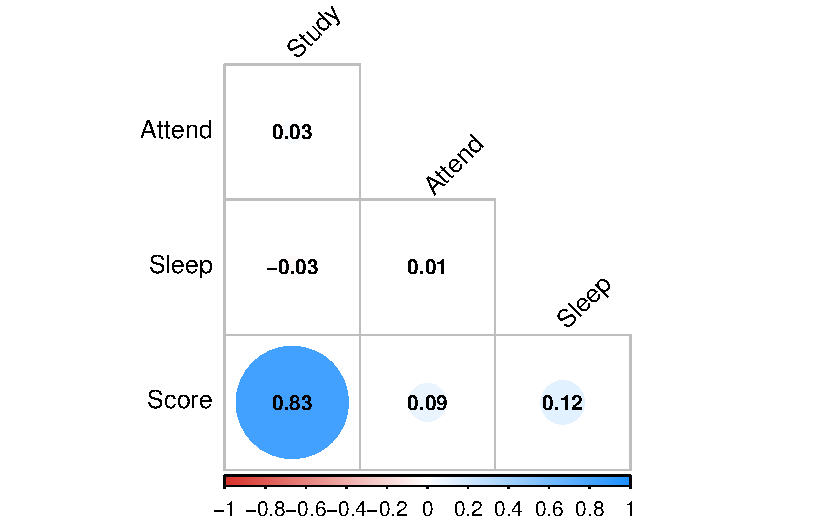
\includegraphics[keepaspectratio]{students-performance-analysis_files/figure-pdf/unnamed-chunk-2-1.pdf}}

\section{Investigating `good' habits'}\label{investigating-good-habits}

\begin{itemize}
\item
  The chart shows how three good habits relate to student exam scores:

  \begin{itemize}
  \tightlist
  \item
    StudyHours, AttendanceRate, and SleepHours.
  \end{itemize}
\item
  \textbf{StudyHours} has a \textbf{strong positive correlation} with
  ExamScore (r = 0.83).

  \begin{itemize}
  \tightlist
  \item
    Students who study more tend to score higher.
  \end{itemize}
\item
  \textbf{AttendanceRate} and \textbf{SleepHours} both show \textbf{weak
  positive correlations}

  \begin{itemize}
  \tightlist
  \item
    Attendance (r = 0.09) and Sleep (r = 0.12) have little impact on
    scores.
  \end{itemize}
\item
  \textbf{Conclusion:} Among the good habits, \textbf{studying
  regularly} is clearly the most effective for better academic
  performance.
\end{itemize}

\begin{Shaded}
\begin{Highlighting}[]
\CommentTok{\# Compute correlation matrix using proper column names}
\NormalTok{bubble\_corr }\OtherTok{\textless{}{-}}\NormalTok{ data\_clean }\SpecialCharTok{|\textgreater{}}
  \FunctionTok{select}\NormalTok{(StudyHours, AttendanceRate, SleepHours, ExamScore) }\SpecialCharTok{|\textgreater{}}
  \FunctionTok{cor}\NormalTok{(}\AttributeTok{use =} \StringTok{"complete.obs"}\NormalTok{)}

\CommentTok{\# Bubble matrix plot with enhanced aesthetics}
\FunctionTok{corrplot}\NormalTok{(}
\NormalTok{  bubble\_corr,}
  \AttributeTok{method =} \StringTok{"circle"}\NormalTok{,}
  \AttributeTok{type =} \StringTok{"lower"}\NormalTok{,}
  \AttributeTok{order =} \StringTok{"hclust"}\NormalTok{,}
  \AttributeTok{tl.col =} \StringTok{"black"}\NormalTok{,}
  \AttributeTok{tl.srt =} \DecValTok{45}\NormalTok{,}
  \AttributeTok{col =} \FunctionTok{colorRampPalette}\NormalTok{(}\FunctionTok{c}\NormalTok{(}\StringTok{"\#d73027"}\NormalTok{, }\StringTok{"white"}\NormalTok{, }\StringTok{"\#1E90FF"}\NormalTok{))(}\DecValTok{200}\NormalTok{),}
  \AttributeTok{addCoef.col =} \StringTok{"black"}\NormalTok{,}
  \AttributeTok{number.cex =} \FloatTok{0.9}\NormalTok{,}
  \AttributeTok{diag =} \ConstantTok{FALSE}
\NormalTok{)}
\end{Highlighting}
\end{Shaded}

\begin{figure}[H]

{\centering \pandocbounded{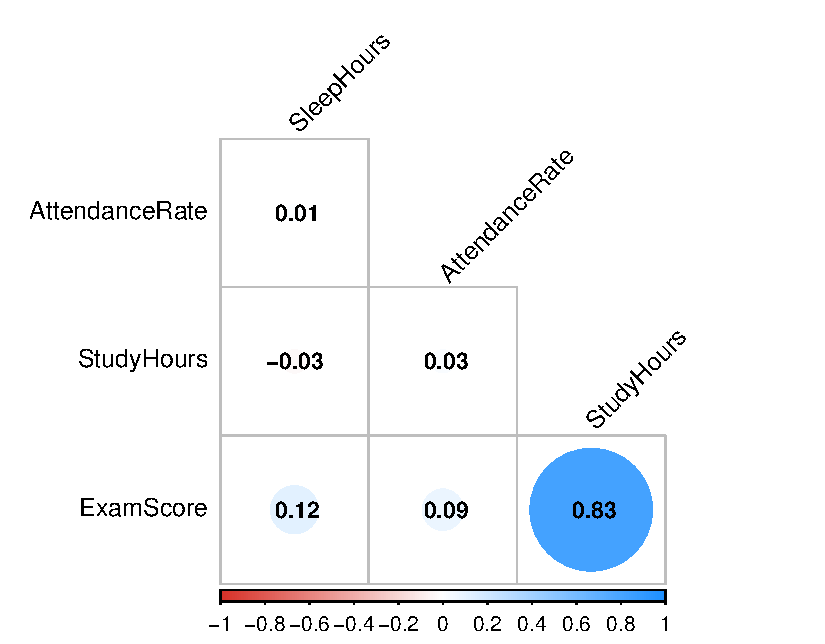
\includegraphics[keepaspectratio]{students-performance-analysis_files/figure-pdf/bubble-corrplot-1.pdf}}

}

\caption{\textbf{Figure 1}: Bubble-style correlation matrix of student
habits and exam score}

\end{figure}%

\newpage

\section{Investigating `bad' habits'}\label{investigating-bad-habits}

\begin{itemize}
\item
  The chart shows how two bad habits relate to exam performance:

  \begin{itemize}
  \tightlist
  \item
    SocialMediaHours and NetflixHours.
  \end{itemize}
\item
  Both habits have \textbf{weak negative correlations} with ExamScore (r
  = -0.17 each).

  \begin{itemize}
  \tightlist
  \item
    More time spent on these may slightly lower scores.
  \end{itemize}
\item
  The two habits are \textbf{not correlated with each other} (r = 0.01).

  \begin{itemize}
  \tightlist
  \item
    Social media and Netflix usage appear to be independent.
  \end{itemize}
\item
  \textbf{Conclusion:} These habits may slightly harm performance, but
  the effect is \textbf{not strong} or highly predictive.
\end{itemize}

\begin{Shaded}
\begin{Highlighting}[]
\CommentTok{\# Create correlation matrix}
\NormalTok{bad\_bubble\_corr }\OtherTok{\textless{}{-}}\NormalTok{ data\_clean }\SpecialCharTok{|\textgreater{}}
  \FunctionTok{select}\NormalTok{(SocialMediaHours, NetflixHours, ExamScore) }\SpecialCharTok{|\textgreater{}}
  \FunctionTok{cor}\NormalTok{(}\AttributeTok{use =} \StringTok{"complete.obs"}\NormalTok{) }\SpecialCharTok{|\textgreater{}}
  \FunctionTok{round}\NormalTok{(}\DecValTok{2}\NormalTok{)}

\CommentTok{\# Rename just for the plot}
\FunctionTok{colnames}\NormalTok{(bad\_bubble\_corr) }\OtherTok{\textless{}{-}} \FunctionTok{c}\NormalTok{(}\StringTok{"Social"}\NormalTok{, }\StringTok{"Netflix"}\NormalTok{, }\StringTok{"Score"}\NormalTok{)}
\FunctionTok{rownames}\NormalTok{(bad\_bubble\_corr) }\OtherTok{\textless{}{-}} \FunctionTok{c}\NormalTok{(}\StringTok{"Social"}\NormalTok{, }\StringTok{"Netflix"}\NormalTok{, }\StringTok{"Score"}\NormalTok{)}

\CommentTok{\# Set margins to avoid clipping}
\FunctionTok{par}\NormalTok{(}\AttributeTok{mar =} \FunctionTok{c}\NormalTok{(}\DecValTok{2}\NormalTok{, }\DecValTok{2}\NormalTok{, }\DecValTok{5}\NormalTok{, }\DecValTok{2}\NormalTok{))  }\CommentTok{\# Add space on top}

\CommentTok{\# Plot}
\FunctionTok{corrplot}\NormalTok{(}
\NormalTok{  bad\_bubble\_corr,}
  \AttributeTok{method =} \StringTok{"circle"}\NormalTok{,}
  \AttributeTok{type =} \StringTok{"lower"}\NormalTok{,}
  \AttributeTok{order =} \StringTok{"original"}\NormalTok{,}
  \AttributeTok{tl.col =} \StringTok{"black"}\NormalTok{,}
  \AttributeTok{tl.srt =} \DecValTok{45}\NormalTok{,}
  \AttributeTok{tl.cex =} \FloatTok{0.9}\NormalTok{,}
  \AttributeTok{cl.cex =} \FloatTok{0.8}\NormalTok{,}
  \AttributeTok{col =} \FunctionTok{colorRampPalette}\NormalTok{(}\FunctionTok{c}\NormalTok{(}\StringTok{"\#d73027"}\NormalTok{, }\StringTok{"white"}\NormalTok{, }\StringTok{"\#1E90FF"}\NormalTok{))(}\DecValTok{200}\NormalTok{),}
  \AttributeTok{addCoef.col =} \StringTok{"black"}\NormalTok{,}
  \AttributeTok{number.cex =} \FloatTok{0.8}\NormalTok{,}
  \AttributeTok{diag =} \ConstantTok{FALSE}
\NormalTok{)}
\end{Highlighting}
\end{Shaded}

\begin{figure}[H]

{\centering \pandocbounded{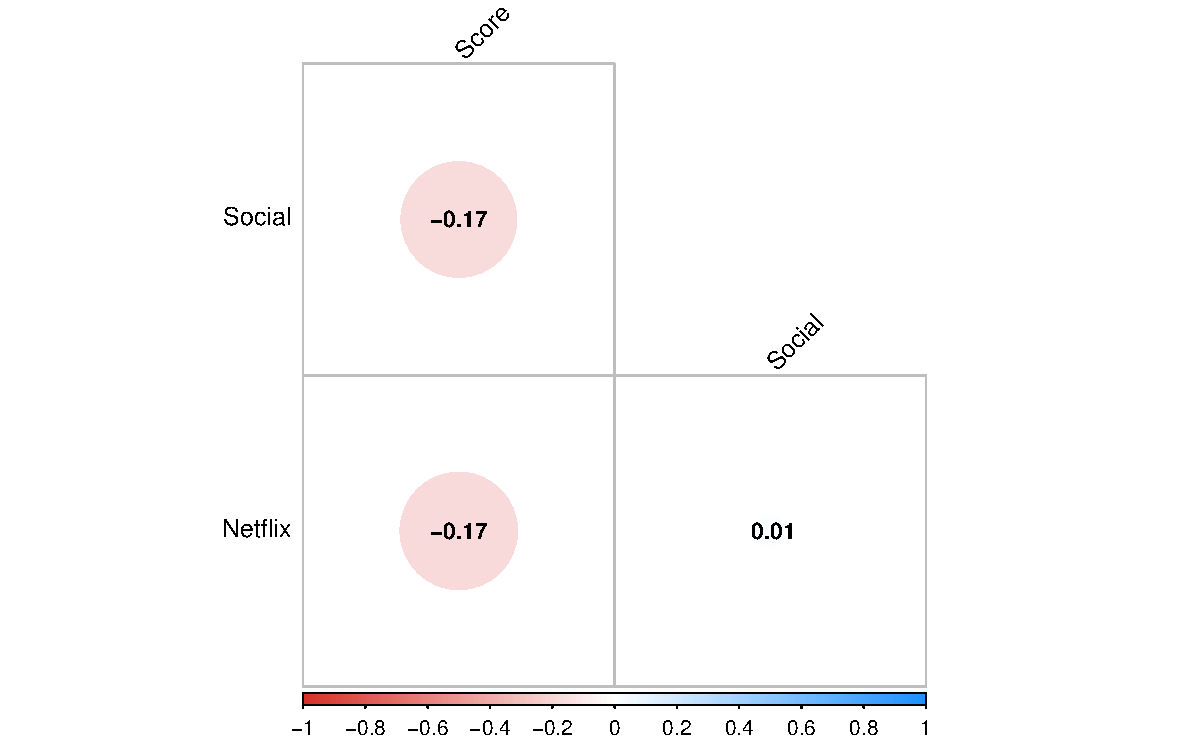
\includegraphics[keepaspectratio]{students-performance-analysis_files/figure-pdf/bubble-corrplot-bad-1.pdf}}

}

\caption{\textbf{Figure 2}: Bubble-style correlation matrix of bad
habits and exam score}

\end{figure}%

\newpage

\section{Results:}\label{results}

The table below summarizes how each lifestyle habit correlates with
academic performance.

\textbf{Table 1} shows that \texttt{StudyHours} has a strong positive
relationship with \texttt{ExamScore} (r = 0.83), making it the most
significant factor influencing academic success. \texttt{AttendanceRate}
(r = 0.09) and \texttt{SleepHours} (r = 0.12) show weak positive
associations, suggesting minor contributions.

In contrast, both \texttt{SocialMediaHours} and \texttt{NetflixHours}
have weak negative correlations with exam scores (r = -0.17 each),
indicating that increased screen time may slightly reduce performance.
However, the strength of these negative relationships is modest and not
highly predictive on their own.

Overall, the results emphasize that consistent study habits are the most
important contributor to higher academic performance, while excessive
media consumption may act as a mild deterrent.

\begin{Shaded}
\begin{Highlighting}[]
\CommentTok{\# Select all habits of interest}
\NormalTok{combined\_corr }\OtherTok{\textless{}{-}}\NormalTok{ data\_clean }\SpecialCharTok{|\textgreater{}}
  \FunctionTok{select}\NormalTok{(StudyHours, AttendanceRate, SleepHours, SocialMediaHours, NetflixHours, ExamScore) }\SpecialCharTok{|\textgreater{}}
  \FunctionTok{cor}\NormalTok{(}\AttributeTok{use =} \StringTok{"complete.obs"}\NormalTok{) }\SpecialCharTok{|\textgreater{}}
  \FunctionTok{round}\NormalTok{(}\DecValTok{2}\NormalTok{)}

\CommentTok{\# Extract only exam score correlations}
\NormalTok{score\_corr }\OtherTok{\textless{}{-}}\NormalTok{ combined\_corr[, }\StringTok{"ExamScore"}\NormalTok{, drop }\OtherTok{=} \ConstantTok{FALSE}\NormalTok{] }\SpecialCharTok{|\textgreater{}}
  \FunctionTok{as.data.frame}\NormalTok{()}
\NormalTok{score\_corr }\OtherTok{\textless{}{-}}\NormalTok{ score\_corr[}\FunctionTok{rownames}\NormalTok{(score\_corr) }\SpecialCharTok{!=} \StringTok{"ExamScore"}\NormalTok{, , drop }\OtherTok{=} \ConstantTok{FALSE}\NormalTok{]}
\FunctionTok{colnames}\NormalTok{(score\_corr) }\OtherTok{\textless{}{-}} \StringTok{"Correlation with ExamScore"}

\FunctionTok{kable}\NormalTok{(score\_corr)}
\end{Highlighting}
\end{Shaded}

\begin{longtable}[]{@{}lr@{}}
\toprule\noalign{}
& Correlation with ExamScore \\
\midrule\noalign{}
\endhead
\bottomrule\noalign{}
\endlastfoot
StudyHours & 0.83 \\
AttendanceRate & 0.09 \\
SleepHours & 0.12 \\
SocialMediaHours & -0.17 \\
NetflixHours & -0.17 \\
\end{longtable}

\newpage

\section{Discussion, Conclusion and
Recommendations:}\label{discussion-conclusion-and-recommendations}

\begin{itemize}
\item
  The findings from this analysis reinforce a key academic principle:
  consistent study habits have the strongest impact on student
  performance. Among all the lifestyle factors examined,
  \texttt{StudyHours} had a clear and substantial correlation with
  \texttt{ExamScore}, while other good habits like
  \texttt{AttendanceRate} and \texttt{SleepHours} played minor roles.
\item
  On the other hand, bad habits such as time spent on social media and
  Netflix showed weak negative correlations with academic performance.
  Although these habits may slightly affect scores, they are not as
  influential as focused study time. This suggests that managing
  distractions is helpful, but not sufficient without active effort
  toward academic preparation.
\item
  From a practical perspective, students should prioritise building
  regular study routines, as this habit alone appears to yield the most
  significant academic benefit. Digital distractions should be monitored
  and managed, but not overly blamed for performance gaps without
  considering time spent studying.
\item
  Future research could explore how motivation, learning environment, or
  time management interact with these habits. Additionally, collecting
  longitudinal data could help identify whether these correlations hold
  consistently over time or vary by context.
\end{itemize}

\# References

\begin{enumerate}
\def\labelenumi{\arabic{enumi}.}
\item
  Dataset: Student Habits and Performance. Simulated dataset for
  academic use, 2025.
\item
  Ian, A., Syam, M. A., \& Rante, A. (2025). The Relationship Between
  Study Hours and Students' Academic Achievement. \emph{SSRN}.
  \url{https://ssrn.com/abstract=5124254}
\item
  Abbas, J., Aman, J., Nurunnabi, M., \& Bano, S. (2023). Association
  between social media use and students' academic performance: A
  structural equation modeling approach. \emph{Education and Information
  Technologies}, 28, 123--145.
  \url{https://link.springer.com/article/10.1007/s10639-023-12407-y}
\end{enumerate}




\end{document}
